\section{Experimentation}

\subsection{rcssserver}
rcssserver is the official simulation environment for the RoboCup SSL tournament. One of the tasks was to get a working strategy to be compatible with rcssserver so that it could be tested in a real game. The Github repository for rcssserver was cloned and set up in a virtual Linux environment by using Ubuntu. The repository for rcssmonitor was also cloned, which is the interface for watching the games in real time. rcssserver games are run by initially connecting to a server to establish a connection between the user's computer and server. Agent movement in the game is then coordinated by the server that receives commands from the connected computer on what each agent should do. The first step was to write the code for connection establishment, which used a simple UDP connection to communicate. Once that was done, the documentation for rcssserver was read to understand built in functions and commands to control the robots. Firstly, a simple program was made to have the agents move into their starting positions. This program was then modified to produce different scenarios. A go-to-ball program was made where the sole purpose was for a single agent to go to the ball and shoot it towards the goal and repeat that once it scored. Each agent ran on their own thread, sending requests and commands to the servers independently for each agent.

\subsection{Strategy Hierarchy}
The following Hierarchy shows how we could organize Team behavior across 5 layers, from high-level strategy down to low-level execution. Each layer builds on the one above it, enabling modular, scalable control.

\begin{figure}[h]
    \centering
    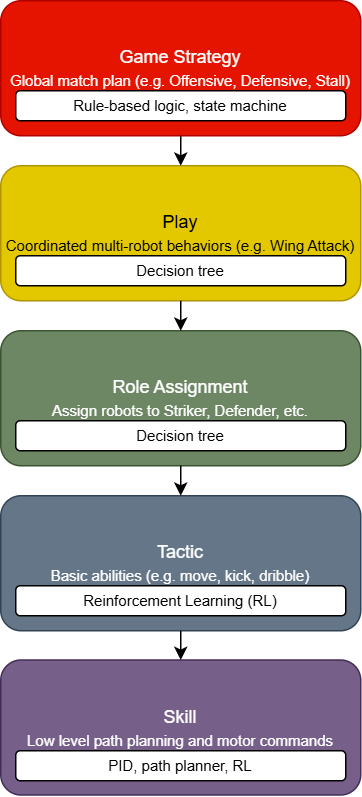
\includegraphics[width=0.8\linewidth]{./StrategyHierarchy.png}
    \caption{Hierarchical team behavior structure}
    \label{fig:strategy_hierarchy}
\end{figure}

\subsubsection{Game Strategy}
The top-layer defines the overall team behavior based on the given game state.
If we take Rule-based logic for example, we could look at time left to play and score.
Then if we are winning and the time is lower than a specified threshold, we could set the Strategy to Stall. This will then provide high-level context for all other decisions made below.

\subsubsection{Play}
The play layer selects coordinated maneuvers such as setting up a wing attack or forming a defensive wall. Selecting plays could be done by a decision tree based on factors like ball position, team formation, and opponent layout. Each play then sets constraints or goals for roles and tactics.

\subsubsection{Role Assignment}
This layer will dynamically assign robots to specific roles (e.g. striker, defender, goalie) based on their position, proximity to the ball, or other factors.
Optimization algorithms such as Hungarian matching have been used with great success.

\subsubsection{Tactic}
The tactic layer defines what action a robot should take in its current role.
This could be whether the robot should pass, dribble, shoot, or intercept.
This layer's decisions are highly context-sensitive and reinforcement learning is a good choice.

\subsubsection{Skill}
The skill layer handles the low-level physical execution of actions.
This could be moving to a position, kicking (how hard) or dribbling. Commonly used control methods are PID and path planning, but reinforcement learning can also be used to improve fine motor control, adaptability, or performance in unpredictable situations.

\subsection{Training}
Part of the training and testing process was conducted using the Virtual Multiagent Simulator. A new simulation model was developed to replicate a football match in the B Division of the Small Size League (SSL). The virtual environment included a field and agent-based robots, all scaled to match real-world dimensions. Key game mechanics such as out-of-bounds, goal-out, and corner detection were implemented. Basic functionalities—such as shooting, passing, positioning, dribbling, opening space, and throw-ins—were also incorporated. Each simulation session lasted 10 minutes, with two teams (red and blue), each consisting of six agents. The red team followed a hardcoded script that selected the first available action, while the blue team was trained to select optimal actions using various AI models, including rule-based systems and reinforcement learning techniques.

\subsection{Agent Architecture: Single vs Multi-Agent}

There are two considered approaches herein when creating AI for multiple agents: single-agent or a multi-agent architecture.

A \textbf{single-agent} approach would involve one central controller that receives the entire field state and outputs coordinated actions for all robots. This method simplifies coordination and is often easier to implement and train.

A \textbf{multi-agent} approach would assign each robot its own agent, possibly with limited field knowledge. This approach is more realistic and can model decentralized behavior, but introduces complexity in coordination and learning stability.

Our initial focus will likely lean toward the single-agent model to reduce complexity during development. However, we may transition to or experiment with a multi-agent setup depending on performance and scalability needs.

\subsection{Reinforcement Learning}
Our main approach involved training a multi-agent reinforcement learning policy for our RoboCup SSL simulation using the VMAS framework, adapted to the RoboCup SSL specifications.  
We used Proximal Policy Optimization (PPO) with a centralized critic.  
We set out to train across multiple scenarios, including ``defensive'', ``ball at centre'', and ``offensive'' scenarios with further differentiation, varying the number of own players and enemy players, the distance to the ball, and the distance to the goal.

The main reason for not just training on full games is that the rewards are more sparse in a full game setup.

It's easier to train agents to shoot a goal when the players are in situations that don't require many actions to shoot a goal.

\subsubsection{PPO Setup}
\textbf{Disclaimer:} Due to ongoing difficulties with our simulator and unreliable shooting mechanics, most work was going into solving those issues and not optimizing parameters, reward function, or varying scenarios.

\begin{itemize}
    \item PPO updates: [e.g., 4 epochs per update, batch size 32, learning rate $1\mathrm{e}{-3}$]
    \item Actions: high-level (move, shoot, pass, dribble), mapped to low-level continuous actions including (dribble direction and speed, shotpower, pass\_scores for each teammate)
    \item Rewards: rewarded for scoring goals, getting closer to the enemy's goal, getting closer to the ball; punished if the other team scores a goal.
\end{itemize}


%\subsection{Continuous action-spaces}
%In the previous section on DQN, the loss function for the network is explained, wherein the action with the largest reward was chosen: \(\underset {a'} {\text{max}} Q(s',a';\theta^-_i)\). This -- as opposed to the case with soccer robots -- presumes the action space to be discrete, finite and meaningfully separate. This prompts a modification to the method suiting our needs. We therefore propose viewing the action space \(\mathcal{A}\) as  !!!!!!!!!!!!!!!!!!!!!!!!!!!!!!!!!!!!!!!!!!!!!!!!!!!!!!!!!!!!!!!!!!!!!!!!!!!!!!!!!!!!!!!!!!!!!!!!!!!!!!!!!!!!!!!!!!!!!!!
